\documentclass{article}
\usepackage[utf8]{inputenc}
\usepackage{fancyhdr}
\usepackage{amsmath}
\usepackage{amsfonts}
\usepackage{amssymb}
\usepackage[left=2cm,right=2cm,top=2cm,bottom=2cm]{geometry}
\usepackage{mathtools}
\usepackage{qtree}
\usepackage{subfiles}
\usepackage{hyperref}
\usepackage{titlesec}
\usepackage{tocloft}

\usepackage{titlepic}
\usepackage{enumitem}
\usepackage{lastpage}
\usepackage{lipsum}
\usepackage{listings}
\usepackage{color}
\usepackage{caption}
\usepackage{subcaption}
\usepackage[font=small]{caption, subcaption}
\usepackage{float}





% Quick correctly proportioned curly brackets
\newcommand{\lr}[1]{\left\{ #1 \right\}}
% Boldsymbol quicker
\newcommand{\bs}[1]{\boldsymbol{ #1 }}

\title{Introduction to skeletonization and implementation of non-embedded distances}
\author{
    Gustav Lang Moesmand (s174169)\\\\
    Supervisors:\\
    Aasa Feragen\\
    Eva Rotenberg\\
    Jakob Andreas Bærentzen
}

\date{
    22 January 2021
}


% Section Thingis
\renewcommand{\cftsecnumwidth}{1em}
%\renewcommand{\thesection}{}
%\renewcommand{\thesubsection}{}
%\renewcommand{\thesubsubsection}{}

% Align Equation commands
\renewcommand{\theequation}{\arabic{equation}}

% Changes symbol around numbering
\newtagform{rightdot}{(}{)}
\usetagform{rightdot}


\pagestyle{fancy}
\fancyhf{}
\lhead{Gustav Moesmand (s174169)}
\chead{Project Plan - Skeletonize Mnist}
\rhead{Bachelor Project}
\rfoot{Page \thepage \hspace{1pt} of \pageref{LastPage}}

\title{Data analysis with skeletons computed from graphs - Project Plan}
\author{Gustav Lang Moesmand (s174169)\\\\\textbf{Supervisors}\\Aasa Feragen, Eva Rotenberg\\ and Jakob Andreas Bærentzen}


\begin{document}
\maketitle

\section{Introduction}
I will in this project plan write my understanding of the premise of the project, the different motivations for investigating the matter, construct a rough roadmap as well as look at general concerns and possible solutions.

\section{Premise}
The premise of the project is to use an implementation of skeletonization of graphs, to model data sets with missing labels, which might yield good results for certain types of data. In the case of this project, the graph will be comprised of a vertex $v$ for every datapoint in the data set, and some edges $e$ modelling the distance between the different datapoints. This distance will most likely be some rough estimation of how alike two points are. As an example, the main dataset that will be used in this project, the Mnist numbers, will have a distance representing how alike two images are in some regard. The implementation of this project will look a little like:

\begin{enumerate}
    \item Create a heurstic for calculating distance 
    \item Create graph from distances. This graph would be a set of vertices $V$ where each vertex $v_i$ would corrospond to a datapoint $d_i$. This graph would then have an edge from each vertex to every other, yielding $i^2$ edges. 
    \item Create skeleton from graph using GEL.
    \item Skeleton should now be able to predict the label of new unlabelled data.
\end{enumerate}
It is very likely, that this will undergo changes, an example might be, that $i^2$ edges is far too many, and a more pragmatic solution is found.

\section{Motivation}
It is expected that this new method in some way will help in modelling variation in data. When modelling data, we usually have some preconception of how the data is shaped, is it linear, is it exponential, a parabel, etc, while the truth might be, that the relation is more complicated. Using the approach of skeletons this bias is eliminated, and we might see that this approach yields good results with data, that locally can be described with a single parameter, showing the dominating trend of the data.
\newpage
\section{Rough roadmap}
\begin{figure}[!h]
    \centering
    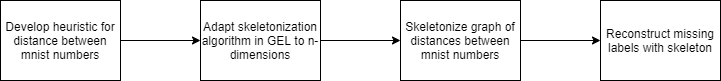
\includegraphics[width=.9\textwidth]{datum/CoarseProjectPlan.png}
\end{figure}


\subsection{Validation of the different phases}
To look at how well the code works, validation of the results from the different phases will be conducted. Below are the current ideas for testing for each step:
\begin{enumerate}
    \item Heuristic: Look at how alike the different distance functions places datapoints with the same label.
    \item Skeletonization: In an n-dimensional embedded room create a structure of vertices and edges. Create noise around the structures vertices and edges, and create a graph from this. Skeletonize the graph and measure the distance between the original structure, and the skeletonized one.
    \item Reconstruction: Look at error rate, how many labels are reconstructed correctly, and how many are wrong.
\end{enumerate}


\section{Expected blockers}
\subsection{Adapting GEL to n-dimensions}
Looking at the code, it has become quite apparent, that there are many parts of the skeletonization algorithm, that relies on other datastructes, also only working in 2-/3-dimensions. I therefore anticipate to use quite some time on this part of the project.

\subsection{Tweaking}
This has already become apparent working with the distance between Mnist numbers, and as a good solution has not yet been found, i expect more time to be used here.

\subsection{The report}
Although this is not included in producing the code, i expect a lot of my time to be used here. The main reason behind this is that a lot of these subjects are in some regard new to me. I do have an underlying intuition, but the bridge between intuition and academic language might take some of my time. 

\end{document}